%% 
%% Copyright 2019-2020 Elsevier Ltd
%% 
%% This file is part of the 'CAS Bundle'.
%% --------------------------------------
%% 
%% It may be distributed under the conditions of the LaTeX Project Public
%% License, either version 1.2 of this license or (at your option) any
%% later version.  The latest version of this license is in
%%    http://www.latex-project.org/lppl.txt
%% and version 1.2 or later is part of all distributions of LaTeX
%% version 1999/12/01 or later.
%% 
%% The list of all files belonging to the 'CAS Bundle' is
%% given in the file `manifest.txt'.
%% 
%% Template article for cas-dc documentclass for 
%% double column output.

%\documentclass[a4paper,fleqn,longmktitle]{cas-dc}
\documentclass[a4paper,fleqn]{cas-dc}

\usepackage[numbers]{natbib}
%\usepackage[authoryear]{natbib}
%\usepackage[authoryear,longnamesfirst]{natbib}

%%%Author definitions
\def\tsc#1{\csdef{#1}{\textsc{\lowercase{#1}}\xspace}}
\tsc{WGM}
\tsc{QE}
\tsc{EP}
\tsc{PMS}
\tsc{BEC}
\tsc{DE}
%%%

% Uncomment and use as if needed
%\newtheorem{theorem}{Theorem}
%\newtheorem{lemma}[theorem]{Lemma}
%\newdefinition{rmk}{Remark}
%\newproof{pf}{Proof}
%\newproof{pot}{Proof of Theorem \ref{thm}}

\begin{document}
\let\WriteBookmarks\relax
\def\floatpagepagefraction{1}
\def\textpagefraction{.001}

% Short title
\shorttitle{Evaluation of cardiac ejection fraction in echocardiograms using a UViT / Roberta neural network}

% Short author
\shortauthors{Carvalho et~al.}

% Main title of the paper
\title [mode = title]{Improving the heart ejection fraction evaluation using a
modified ultrasound Vision Transformer architecture}                      
% Title footnote mark
% eg: \tnotemark[1]


% Title footnote 1.
% eg: \tnotetext[1]{Title footnote text}
% \tnotetext[<tnote number>]{<tnote text>} 



% First author
%
% Options: Use if required
% eg: \author[1,3]{Author Name}[type=editor,
%       style=chinese,
%       auid=000,
%       bioid=1,
%       prefix=Sir,
%       orcid=0000-0000-0000-0000,
%       facebook=<facebook id>,
%       twitter=<twitter id>,
%       linkedin=<linkedin id>,
%       gplus=<gplus id>]


\author[1]{Thiago Carvalho}

% Corresponding author indication
\cormark[1]

% Footnote of the first author
\fnmark[1]

% Email id of the first author
\ead{thiago.augustocarvalho@gmail.com}

% URL of the first author
%\ead[url]{www.cvr.cc, cvr@sayahna.org}

%  Credit authorship
%\credit{Conceptualization of this study, Methodology, Software}

% Address/affiliation
\affiliation[1]{organization={Computing Institute, Universidade Federal Fluminense},
    addressline={Av. Gal. Milton Tavares de Souza, s/n São Domingos}, 
    city={Niteroi},
    % citysep={}, % Uncomment if no comma needed between city and postcode
    postcode={24210-346}, 
    state={Rio de Janeiro},
    country={Brazil}}



% Third author
\author[1]{Flavio Luiz Seixas}
\fnmark[2]
\ead{claudiotinocomesquita@id.uff.br}

% Address/affiliation
\affiliation[2]{organization={Medical School, Universidade Federal Fluminense},
    addressline={Av. Marquês do Paraná, 303 - Centro}, 
    city={Niteroi},
    % citysep={}, % Uncomment if no comma needed between city and postcode
    postcode={24033-900}, 
    state={Rio de Janeiro},
    country={Brazil}}

% Here goes the abstract
\begin{abstract}
In this article addressed the need for more reliable cardiac diagnoses, crucial for effective treatments of various heart conditions, and focused on optimizing echocardiogram analysis methods to improve the accuracy of left ventricular ejection fraction estimation, which is essential for cardiac diagnoses. After a systematic literature review and the selection of adult and pediatric echocardiogram datasets, the methodology utilized a modified version of the Ultrasound Video Transformer (UViT), integrating technologies such as RoBERTa for spatiotemporal analysis. The evaluation of the models, using metrics like MAE, RMSE, and R², revealed significant improvements compared to the reviewed literature, especially with the RoBERTa model, which excelled in terms of accuracy and generalization capacity for both adult and pediatric data. The research suggests that the proposed approach can enhance diagnostic accuracy and be clinically applied, contributing to more informed medical decisions. The contributions include a robust method for echocardiogram analysis and pave the way for future work in automatic patient categorization by age, improving image quality with generative neural networks, and automatic interpretation of medical reports with advanced language models.

\end{abstract}

% Use if graphical abstract is present
% \begin{graphicalabstract}
% 
\includegraphics{figs/grabs.pdf}
% \end{graphicalabstract}

% Research highlights
\begin{highlights}
\item This manuscript shows a modified Ultrasound Vision Transformer architecture for calculating the left ventricular ejection using echocardiogram images.
\item We evaluate the results using Echonet and Echoped datasets, showing upper results than recent publications.
\item A computational system applied to aid physicians in diagnosing and treating patients with heart failure.
\end{highlights}

% Keywords
% Each keyword is seperated by \sep
\begin{keywords}
Left ventricular ejection fraction \sep Ultrasound Vision Transformer architecture \sep Heart failure \sep Echocardiography \sep Artificial Intelligence
\end{keywords}

\maketitle

\section{Introduction}

Cardiovascular diseases, which include conditions such as coronary artery disease, hypertension, heart failure, and stroke, have a significant impact not only on individuals' physical quality of life but also generate highly relevant repercussions in social, economic, and health domains \cite{Stevens2018}. The \textit{Global Burden of Disease} 2019 report confirms this impact, identifying cardiovascular diseases as the leading cause of death worldwide, which illustrates the magnitude of the challenge these conditions represent for global health \cite{https://doi.org/10.6069/1d4y-yq37}.
In the Brazilian context, the economic implications are particularly notable. Cardiovascular diseases account for 28% of all deaths in Brazil, with estimated costs reaching R$ 37.1 billion in 2015. Of this total, premature deaths represent 61%, direct costs with hospitalizations and consultations account for 22%, and productivity loss amounts to 15%. With health spending in Brazil estimated at 9.5% of GDP, cardiovascular diseases consume approximately 0.7% of GDP \cite{Siqueira2017}. These findings underscore the importance of effective prevention and control measures, not only for population health but also for the country's economic stability.
To address these challenges, the introduction of echocardiography in the 1970s marked a significant milestone in cardiovascular disease diagnosis, bringing substantial advances and enabling more precise and effective approaches \cite{haley_2018}. This low-cost, minimally invasive technique has become widely accessible, offering crucial information for managing numerous cardiovascular conditions \cite{Mancuso2014}. Echocardiography plays a fundamental role as a multidisciplinary tool in the diagnosis and prognostic evaluation of acute coronary syndromes, heart failure, and other cardiac conditions, while also being essential for determining appropriate treatment in patients with cardiac arrhythmias \cite{Mancuso2014}.
Despite these advances, limitations remain. While portable echocardiography devices now allow examination of cardiac functionality outside clinical settings with real-time imaging capabilities \cite{Xiao}, result interpretation still depends heavily on operator experience, potentially leading to variations and diagnostic errors. To overcome this limitation, Artificial Intelligence (AI) has emerged as a promising solution to make echocardiogram interpretations more accurate, consistent, and automated, thereby minimizing human error risks and improving diagnostic quality \cite{Alsharqi2018}.
Within cardiac assessment metrics, the Left Ventricular Ejection Fraction (LVEF) stands as a fundamental parameter for diagnosing cardiac pathologies, offering significant prognostic value in predicting adverse outcomes in heart failure patients \cite{kosaraju_grigorova_goyal_makaryus}. However, accurate LVEF extraction presents considerable challenges due to the necessity of selecting high-quality frames during Diastole (D) and Systole (S) phases, a process vulnerable to inter- and intra-observer variability errors \cite{Ouyang2020}.
While machine learning applications in biomedical image analysis have advanced remarkably in recent years, echocardiogram video stream processing continues to face specific challenges. Chief among these is the scarcity of openly available and properly annotated medical video data, creating significant obstacles for developing more accurate analysis techniques \cite{Ouyang2020}. These challenges necessitate innovative approaches to improve LVEF measurement accuracy and reliability.
Given this context, this study aims to improve diagnostic accuracy in cardiology, provide operator support, and effectively address the clinical needs of diverse patients. Our methodology includes a systematic review to identify effective methods and gaps in LVEF measurement, followed by the selection and refinement of a promising model. The enhancement process focuses on identifying and overcoming the model's specific limitations to increase accuracy and generalization in LVEF estimation. To ensure broad clinical applicability, we test the enhanced model's validity and effectiveness through analysis of clinical data from both adult and pediatric patients.
The main contribution of this paper lies in introducing and applying a comprehensive evaluation and experimentation methodology using artificial neural network models for echocardiogram analysis. We propose specific adaptations to existing neural network architectures, alongside careful hyperparameter optimization, to improve precision and robustness in LVEF estimation. Furthermore, we detail the development of an automated pipeline incorporating data preprocessing, model training, cross-validation, and performance analysis, ensuring the trained models achieve both accuracy and generalizability across various clinical contexts.

This article is structured as follows: Chapter \ref{Fundamentação teórica} covers key topics in cardiology and technology, including heart anatomy and physiology, ultrasound, echocardiography, and an introduction to artificial neural networks. Chapter \ref{Revisão bibliográfica} explores the application of deep neural networks in cardiac function assessment using echocardiogram videos, describing the systematic literature review methodology and discussing selected studies. Chapter \ref{Metodologia} details the methodological process for improving echocardiogram analysis, addressing experiment descriptions, database descriptions, implementation of the modified architecture, and parameter optimization. Chapter \ref{sec} presents and discusses the results of experiments with classical and modified models, testing the hypothesis of model generalization. Finally, Chapter \ref{sec ão} concludes by reviewing the main findings, highlighting the improvement in echocardiogram analysis accuracy for calculating Left Ventricular Ejection Fraction (LVEF), discussing clinical implications, study limitations, and suggesting directions for future work.

This article is organized as follows: Section \ref{sec:2} provides an overview of left ventricular ejection calculation methods and machine learning architectures. The design of the proposed architecture is described in Section \ref{sec:3}, followed by results in Section \ref{sec:4}. Finally, Section \ref{sec:5} contains the conclusion.

\section{Foundation and Related Work.} \label{sec:2}

Subsection 2.1 provides the foundation for ejection fraction and its importance in medical diagnosis, while Subsection 2.2 lists the main architectures in the literature for calculating the left ventricular ejection fraction of the heart.

\subsection{Ejection fraction in echocardiogram images.}

The heart is a vital organ responsible for pumping blood through the cardiovascular system. It is composed of four chambers: the right atrium, responsible for receiving blood from the veins and sending it to the right ventricle; the right ventricle, which receives blood from the right atrium and sends it to the lungs; the left atrium, which receives oxygenated blood from the lungs and sends it to the left ventricle; and finally, the left ventricle, which is responsible for pumping oxygen-rich blood throughout the body and thus maintaining adequate blood pressure \cite{hoffman}.

The echocardiogram is a non-invasive, widely available, and low-cost test, and it is widely used in clinical practice to assess heart diseases, determine the size of the heart chambers, ventricular mass, valvular diseases, and hemodynamics \cite{8520425232}.

The left ventricular ejection fraction is an important measure of the heart's contractile function and is calculated by the relationship between the volume of blood ejected in systole and the volume of blood present in the ventricle at the end diastole. The Left Ventricular Ejection Fraction (LVEF) is widely used in the assessment of heart diseases and is classified as normal (55\%), close to normal (45-55\%), moderately abnormal (30-45\%), and markedly abnormal (\textless30\%). The calculation of LVEF is performed from the estimates of the end-diastolic volume (EDV) and the end-systolic volume (ESV), using the equation: $LVEF = (EDV - ESV)/EDV$. The EDV corresponds to the volume of blood present in the left ventricular chamber at the end of diastole, the period of cardiac relaxation, while the ESV represents the volume of blood present in the left ventricular chamber at the end of systole, the period of cardiac contraction \cite{Lang2015}.

To ensure accurate measurements of the left ventricular ejection fraction (LVEF) using echocardiography, specific steps must be followed. The operator needs to obtain apical 4 and 2 chamber images, carefully observe apical shortening and endocardial dropout, and utilize the Simpson technique for precise measurements of LVEF and left ventricular volumes. Apical 4-chamber cuts provide a comprehensive view of the four cardiac chambers and their movements, while apical 2-chamber cuts offer a detailed perspective on the anatomy and movements of the left ventricle \cite{2021}. Figure \ref{FIG:33} displays an illustration of a heart with an apical 4-chamber view.

\begin{figure}
	\centering
		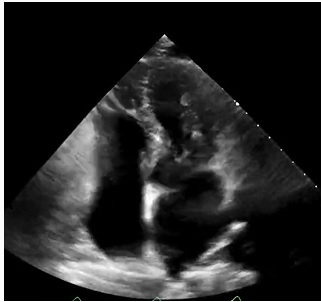
\includegraphics[scale=.75]{saidaa.png}
	\caption{Apical 4-chamber view \cite{Ouyang2019}.}
	\label{FIG:33}
\end{figure}



\subsection{Deep learning architectures.}

In this section, we discuss two widely used deep learning architectures: Convolutional Neural Networks (CNNs) and Transformers for calculating the left ventricular ejection fraction of the heart.

\subsubsection{Convolutional Neural Networks}

Convolutional Neural Networks (CNNs) are deep neural networks widely used in image processing and pattern recognition. The basic architecture of a CNN consists of several layers of elements that perform the convolution operation, followed by pooling and fully connected layers. The convolutional layers are responsible for extracting features from an image, while the pooling layers reduce the dimensionality of the image and preserve the most important features. The fully connected layers use the features extracted by the convolutional and pooling layers to classify the images. CNNs are trained using supervised learning algorithms that adjust the weights and biases of the network to minimize classification error \cite{IZADKHAH2022175}.

CNNs have a wide range of applications in various areas, such as image recognition, object detection, speech recognition, and natural language processing. In the medical field, CNNs are used to analyze medical images and assist in diagnosing diseases. For example, CNNs are used to analyze magnetic resonance imaging and detect brain tumors with high accuracy. CNNs are also used to analyze echocardiogram images and estimate the left ventricular ejection fraction, which can help diagnose and treat heart diseases \cite{IZADKHAH2022175, HE2022}.

\subsubsection{Transformers}

Transformers are a deep neural network architecture that utilizes the self-attention mechanism for sequence processing, originally proposed for Natural Language Processing tasks. They gained prominence by achieving remarkable results in machine translation and text analysis tasks. More recently, the Transformers architecture has been applied to computer vision tasks, such as object detection and image classification, with promising results \cite{RUAN20221}.

The self-attention mechanism is a technique that allows the computation of global representations and dependencies in a dataset, enabling each element in a sequence to interact with all other elements in the sequence instead of relying only on previous or subsequent elements. This process is accomplished by calculating attention weights for each element in the sequence, which are used to weigh the relative importance of each element in computing the final representation. The self-attention mechanism has proven to be very efficient in Natural Language Processing and Computer Vision tasks, allowing the development of pre-trained models with state-of-the-art performance in various data classification and generation tasks \cite{RUAN20221}.

Notable language transformer models include BERT, which is a bidirectional model capable of understanding the context of a word both to the left and right \cite{https://doi.org/10.48550/arxiv.1810.04805}. Its derivatives, such as RoBERTa, aim to improve BERT's capabilities through training with more data or optimization techniques \cite{Roberta,DistilBERT}. Another model is GPT, which is unidirectional and pre-trained to generate natural text \cite{https://doi.org/10.48550/arxiv.2005.14165}.

Furthermore, the \textit{Vision Transformer (ViT)} is a transformer-based neural network architecture designed to handle computer vision tasks. Unlike traditional approaches that use convolutional layers to extract visual features from images, the ViT architecture consists of an initial tokenization layer, which transforms image patches into tokens, followed by several Transformer layers that model the relationships between the tokens. The output of the last Transformer layer is used as input for a linear layer and a softmax layer, which are used to perform image classification \cite{https://doi.org/10.48550/arxiv.2010.11929}.

\subsection{Related Work}

Numerous approaches to calculating heart ejection will be addressed in this section, such as the use of convolutional networks and ViT (Vision Transformer).

EchoNet-Dynamic is a deep-learning algorithm developed for cardiac function assessment. This model can accurately segment the left ventricle, predict ejection fraction, and classify heart failure with reduced ejection fraction with high accuracy. The three main components of the model are $(1)$ left ventricular segmentation, $(2)$ ejection fraction prediction from sub-sampled clips, and $(3)$ cardiomyopathy assessment with beat-to-beat predictions. The algorithm uses a CNN model with atrous convolutions to segment the left ventricle in echocardiogram videos. The labels of the work are generalized in a weak supervision approach to generate semantic segmentation throughout the cardiac cycle. This helps identify ventricular contractions and provides an interpretable intermediary for physicians. The dataset provides 10,030 annotated echocardiogram videos and is publicly available \cite{Ouyang2019}.

EchoNet-Peds describes a deep-learning method for assessing pediatric patients' left ventricular ejection fraction using echocardiogram videos. The proposed method uses a convolutional neural network model to extract features from video frames and a linear regression model to estimate the left ventricular ejection fraction of the heart. The study compared the performance of the proposed method with that of human experts and with other existing deep learning approaches, showing that the proposed method has comparable or superior performance to human experts. The study concludes that the proposed method may be useful for clinical assessment of LVEF in pediatric patients. Like EchoNet-Dynamic, the dataset provides 7,000 annotated pediatric echocardiogram videos and is publicly available \cite{Reddy2023}.

The RVENet model was created with the purpose of assessing right ventricular function with the help of deep learning. A high-quality echocardiographic image dataset was developed, allowing the modeling of a spatiotemporal convolutional neural network (CNN). This specific CNN technique is capable of processing distributed spatial and temporal information, such as videos and temporal image sequences, like echocardiogram medical images. The dataset used in RVENet contains 3,583 2D apical four-chamber echocardiographic videos from 944 transthoracic echocardiographic exams of 831 individuals \cite{10.1007/978-3-031-25066-8_33}.

The work presented \cite{Reynald} introduces a deep learning approach called UViT to estimate left ventricular ejection fraction (LVEF) from echocardiogram video streams. The approach combines using a transformer architecture based on a Self-Encoder Residual Network and a BERT model adapted for token classification. This allows videos of any size to be processed. UViT outperformed the performance of other deep learning methods on the EchoNet-Dynamic dataset, with an MAE (Mean Squared Error) of 5.95 and an R² (a measure of how well the model fits the data) of 0.52 in 0.15s per video.

The use of Transformer models in ultrasound videos for medical image analysis is a promising and innovative approach. Although different from the techniques used in related works, it shares the need for large annotated datasets and the adaptation of the model architecture to handle ultrasound video data. Related works have shown that using deep learning techniques in echocardiogram videos provides accurate and high-quality results.

\section{Neural Network Architecture and Training Dataset} \label{sec:3}

This section presents the materials and methods used to solve the proposed problem. The methodology adopted consists of training and validating a UViT neural network and its modification using the RoBERTa architectures to calculate the heart ejection fraction in adult and pediatric patients. Section \ref{sub:UViT Architecture} describes the original solution used as a reference, while Section \ref{sub:Modified UViT Architecture} presents the rationale for the modifications made and the set of parameters and hyperparameters used. In Section \ref{sub:Training dataset}, the datasets used in this work are demonstrated, and in Section \ref{sub:Implementation}, all the details of the computational environment used are presented.

\subsection{UViT Architecture} \label{sub:UViT Architecture}

The adopted approach was the UViT with a transformer architecture based on a Self-Encoder Residual Network and a BERT model as the foundation for conducting experiments.

The original approach consists of three modules: an encoder, a BERT-based module that provides spatiotemporal reasoning capabilities, and two regressors. The first regressor is responsible for labeling ES (refers to the early systole phase of the cardiac cycle, also known as atrial systole) and ED (refers to the late diastole phase of the cardiac cycle) known as ventricular diastole) frames. The second regressor is used to estimate the left ventricular ejection fraction (LVEF) \cite{Reynald}.

In order to address the computational complexity of the problem, a dimensionality reduction technique was employed using the encoding part of a ResNetAE. This process involves embedding the information from ultrasound frames into a lower-dimensional space by utilizing residual blocks at different scales. The parameters of the model are optimized through reconstruction tasks on a dedicated ultrasound dataset. Subsequently, the embedded frames are transformed into a 1024-dimensional vector and inputted into the Transformer model with BERT for accurate estimation of the left ventricular ejection fraction of the heart \cite{Reynald}. The entire pipeline of the architecture is depicted in Figure \ref{FIG:1}.

o address the computational complexity of the problem, we employed a dimensionality reduction technique using the encoding part of a ResNetAE. This technique enables us to embed the ultrasound frame information into a lower-dimensional space by utilizing residual blocks at multiple scales. By optimizing the model parameters through reconstruction tasks on a dedicated ultrasound dataset, we ensure accurate representation of the latent features. Subsequently, the embedded frames are transformed into a 1024-dimensional vector and inputted into the Transformer model with BERT for precise estimation of the left ventricular ejection fraction of the heart \cite{Reynald}. The entire pipeline of the proposed architecture, including the ResNetAE encoding, BERT processing, and branching into optional SD and EF directions, is depicted in Figure \ref{FIG:1}.

\begin{figure}
	\centering
		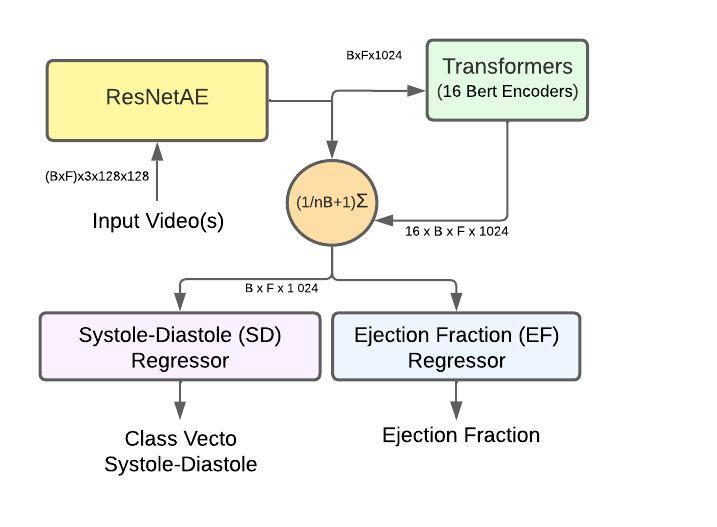
\includegraphics[scale=.75]{Diagrama em branco (1).jpeg}
	\caption{Architecture pipeline for LVEF estimation using ResNetAE and BERT.}
	\label{FIG:1}
\end{figure}

\subsection{Modified UViT Architecture} \label{sub:Modified UViT Architecture}

In this work, two transformer-based models were used: RoBERTa and DistilBERT. RoBERTa is an optimized version of BERT, which achieved superior results in various natural language understanding tasks. DistilBERT is a compact and efficient version of BERT, which maintains high accuracy in text classification tasks and named entity extraction. Both models can be adapted to domains and tasks using simple fine-tuning or task-based distillation techniques \cite{Roberta, DBLP:journals/corr/abs-1910-01108}.

The models were used to determine the heart ejection fraction of adult and pediatric ultrasound videos. To compare the performance of the two models in the emotion recognition task, modifications were made to the original UViT Transformer architecture to accommodate RoBERTa and DistilBERT.

To improve the performance of the new model compared to the original, some changes were made to the hyperparameters. The 'Attention Heads' parameter, which determines the number of attention heads used in each Transformer layer for detailed and accurate information processing, was increased from 16 to 32. The 'Number of Hidden Layers' was increased from 16 to 32, allowing for a more complex representation of the data. The 'Batch Size' was doubled to 2, speeding up the training process and avoiding overfitting. To prevent GPU memory issues, the 'Max Length (dsmax)' parameter was adjusted from 128 to 64, limiting the maximum number of frames allowed in each video sequence during model training. These changes in the hyperparameters can impact the performance and efficiency of the model, as shown in Table \ref{tbla1}.



\begin{table}[width=.9\linewidth,cols=4,pos=h]
\caption{Comparison of Hyperparameters.}\label{tbla1}
\begin{tabular*}{\tblwidth}{@{} LLLL@{} }
\toprule
Hyperparameter& Original&  Modified \\
\midrule
Number of Hidden Layers & 16       & 32       \\
Attention Heads         & 16       & 32       \\
Batch Size              & 1        & 2        \\
Max Length (dsmax)      & 128      & 64       \\
Epochs                  & 5        & 50     \\ 
\bottomrule
\end{tabular*}
\end{table}


The metrics used to evaluate the models were as follows:

\begin{itemize}
\item The average distance in frames between the predicted frame and the actual frame of the end of systole (ES) and the end of diastole (ED), which are the key points for calculating the ejection fraction.
\item The mean absolute error (MAE) and the coefficient of determination $(R^2)$ between the predicted ejection fraction and the actual ejection fraction, which measure the accuracy and correlation of the method.
\end{itemize}

To demonstrate the generalization of the proposal, data from adult and pediatric patient videos were used, and the performance evaluation of the models will be described in Section \ref{sec:4}. The use of datasets from different age groups allowed us to verify if the proposed technique can handle significant variations in ultrasound video features, which increases the reliability and applicability of the obtained results.

\subsection{Training Dataset} \label{sub:Training Dataset}

The datasets used for training were extracted from two public access databases and described in the following articles:

\begin{itemize}
\item The \textit{EchoNet-Peds} database contains 7,643 echocardiogram videos with labels and annotations made by human specialists, including measurements, traces, and calculations. This database provides a baseline for studying cardiac motion and chamber sizes in patients aged 0 to 18 years, with 43% female and a wide variety of sizes \cite{Reddy2023}.
\item The \textit{EchoNet-Dynamic} database includes 10,030 labeled echocardiogram videos and annotations from human specialists (measurements, traces, and calculations) to provide a baseline for studying cardiac motion and chamber sizes \cite{Ouyang2019}.
\end{itemize}

\subsection{Implementation} \label{sub:Implementation}

All runs were performed in Python, using the PyTorch and transformers libraries, as well as parallel processing with 8 Tesla Pascal GPU cards (model P100-SXM2-16GB) with 16GB and 3584 CUDA cores each, totaling 28,672 CUDA cores. The machine also has 2 Intel Xeon E5-2698 v4 CPUs, 20 cores and 40 threads per CPU, totaling 40 physical or 80 logical cores, 512 GB of RAM, and a 7TB SSD-based data storage. The use of parallel processing on GPUs was a strategy adopted to optimize tasks and reduce computational time.

\section{Results} \label{sec:4}

This session presents the results obtained from the training and validation of the networks, including performance values.

\subsection{UViT Architecture}

The initial experiment used the classic UViT architecture, described in section \ref{sub:UViT Architecture}. Table \ref{exTable1} presents the model's performance on the training and test sets. A slight improvement of 0.84\% was observed in performance compared to Reynaud \textit{et al.}'s work (2021) and the Echonet data on our machine. However, for the Echoped data, although there is no reference for comparison to pediatric data in Reynaud \textit{et al.}'s work (2021), when testing the classic UViT, a lower performance was found compared to Reddy \textit{et al.}'s work (2023).


In comparison to the results of Ouyang \textit{et al.} (2019), Reynaud \textit{et al.} (2021) highlighted that the compared work was divided into two experiments: Echonet (1) and Echonet (2), with different results. While Echonet (1) is restricted by the use of segmentations and a fixed number of frames per beat, aggregating predictions per beat into a final estimate for entire sequences, the processing time is 1.6 seconds per beat and a minimum number of frames, for example, 32, must be available for each beat during retrospective analysis. Echonet (2), on the other hand, uses segmentation and all available frames in a single selected beat without any additional processing. In contrast, the UViT uses the entire video stream without the need for segmentations, making it faster and more efficient. The average processing time of the UViT is 0.15 seconds for complete videos, and the method is capable of performing real-time evaluation during the exam. Table \ref{tab:exTable2} shows that the UViT had superior performance compared to the Echonet (2) results from Ouyang \textit{et al.}'s work (2019).




\begin{table}[width=.9\linewidth,cols=4,pos=h]
\caption{Comparison of Hyperparameters.}\label{exTable1}
\begin{tabular*}{\tblwidth}{@{} LLLLLL@{} }
\toprule
& Paper & Database & &Metrics   &  &\\ \hline
& &  & MAE & RMSE & $R^2$ \\ 
\midrule
1 & \cite{Reynald} & Echonet & 5.88 & 8.38 & 0.51  \\
2 & \cite{Reynald}  & Echoped & 6.23 & 8.92 & 0.82  \\ 
3 & \cite{Ouyang2019} & Echonet & 7.35 & 9.53 & 0.40  \\ 
4 & \cite{Ouyang2019} & Echonet & 4.22 & 5.56 & 0.79  \\ 
5 & \cite{Reddy2023}. & Echoped & 3.66 & - & 0.77  \\ \hline
\bottomrule
\end{tabular*}
\end{table}




\subsection{Modified UViT Architecture}

The second experiment was performed using the modified UViT architecture described in section \ref{sub:Modified UViT Architecture}. Table \ref{exTable3} shows the performance of the proposed model for the training and test data, respectively.

The results obtained using the RoBERTa model demonstrated a 17.68\% increase in performance compared to the original approach by Reynaud et al. (2021), while with the DistilBERT model there was a decrease of 2.21\%. The average processing time also showed differences, being 0.09 for RoBERTa and 0.13 for DistilBERT. Regarding pediatric data, a drop in performance was observed compared to the results obtained for adults in both algorithms. However, the average processing rate remained at 0.09 for RoBERTa and 0.13 for DistilBERT, compared to 0.06 of Reddy et al.'s proposal (2023). This drop in performance can be explained by physiological and anatomical differences between children and adults, which may affect the accuracy of the models in assessing cardiac function. Furthermore, it is important to note that the separation of pediatric data was not carried out considering the age and gender of the patients, which may have influenced the results obtained by the models. The modified architecture used in the study showed significant improvements in performance compared to the original approach by Reynaud et al. (2021) and other proposals. This may have been due to a combination of factors, such as using a more advanced language model, architectural complexity, and processing time optimization with hyperparameters.


\begin{table}[width=.9\linewidth,cols=4,pos=h]
\caption{Modified UViT Ejection Fraction Results}\label{exTable3}
\begin{tabular*}{\tblwidth}{@{} LLLLLL@{} }
\toprule
& Paper & Database & &Metrics   &  &\\ \hline
& &  & MAE \quad & RMSE\quad  & \quad$R^2$  \\ 
\midrule
1 & UivT \cite{Reynald}. & Echonet & 5.88 & 8.38 & 0.51  \\ 
2 & UivT Destilbert  & Echonet & 6.01 & 8.24 & 0.65  \\ 
3 & UivT Roberta & Echonet & 4.84 & 6.32 & 0.47  \\ 
4 & UivT Destilbert  & Echoped & 6.89 & 8.89 & 0.91  \\ 
5 & UivT Roberta & Echoped & 5.72 & 7.23 & 0.67  \\ 
6 & \cite{Ouyang2019} & Echoped & 3.66 & - & 0.77  \\ \hline
\bottomrule
\end{tabular*}
\raggedright \textit{Increasing the number of attention heads and hidden layers allows for a richer and more complex representation of the data. Doubling the batch size speeds up training and helps prevent overfitting. Adjusting the 'Max Length (dsmax)' to 64 helps avoid GPU memory issues.}
\end{table}

In Figure \ref{FIG:2}, we show the prediction results obtained by using the Roberta Transformer model with variations in hyperparameters.

\begin{figure}
	\centering
		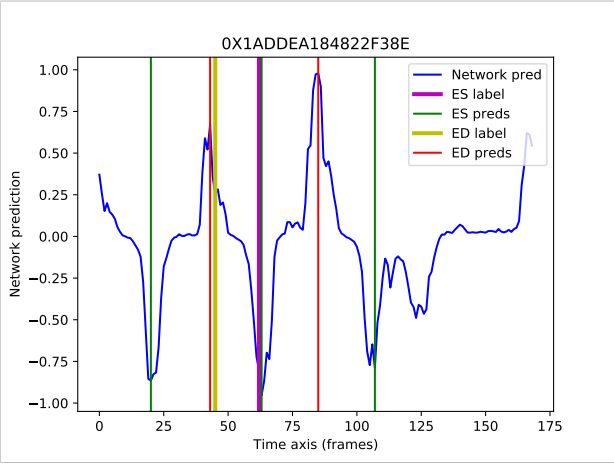
\includegraphics[scale=.60]{saida1.png}
	\caption{The figure illustrates the prediction output of the model in relation to the frames. We can observe the systole label represented by a purple line and the systole predicted by the model shown as a green line. Similarly, the diastole detection is represented by a yellow line by the medical operator and a red line by the proposed model.}
	\label{FIG:2}
\end{figure}



\section{Conclusion} \label{sec:5}

Our work presented an improved approach for calculating the left ventricular ejection fraction of the heart, which achieved promising results in terms of accuracy and processing time in adult and pediatric data. Modifications to the UViT network, such as introducing new hyperparameters and using Bert model variations, allowed for improved performance and avoided overfitting issues. However, further studies are needed to refine the applicability of the approach in different age ranges, such as dividing the pediatric dataset into age and sex groups and including data from different echocardiogram video captures to assess cardiac function and heart anatomy. and heart anatomy. It is hoped that this approach can be
applied to other areas of  applied to other areas of medicine dealing with temporal image data, contributing to advancements in diagnosing and treating cardiovascular diseases.


%% Loading bibliography style file
%\bibliographystyle{model1-num-names}
%\bibliographystyle{cas-model2-names}

\bibliographystyle{elsarticle-num} 

% Loading bibliography database
\bibliography{cas-refs}


\end{document}

